\chapter{RESULTS AND ANALYSIS}


\section{Baseline Model Comparison}


\begin{table}[H]
    \centering
    \small
    \caption{Baseline Model Comparison}
    \label{tab:baseline_model_comparison}
    \renewcommand{\arraystretch}{1.2}
    \begin{tabularx}{0.94\linewidth}{|X|X|X|X|}
        \hline
        \textbf{Model} & \textbf{MAE} & \textbf{RMSE} & \textbf{$R^2$} \\
        \hline
        Persistence baseline & 6.723 & 10.500 & 0.708 \\
        \hline
        Linear Regression (OLS, all features) & 21.091 & 24.116 & -2.982 \\
        \hline
        Ridge Regression, all features ($\alpha$=10) & 10.000 & 13.257 & 0.415 \\
        \hline
        \textbf{Ridge Regression, pruned features ($\alpha$=10)} & \textbf{9.575} & \textbf{12.846} & \textbf{0.448} \\
        \hline
    \end{tabularx}
\end{table}


\begin{figure}[H]
    \centering
    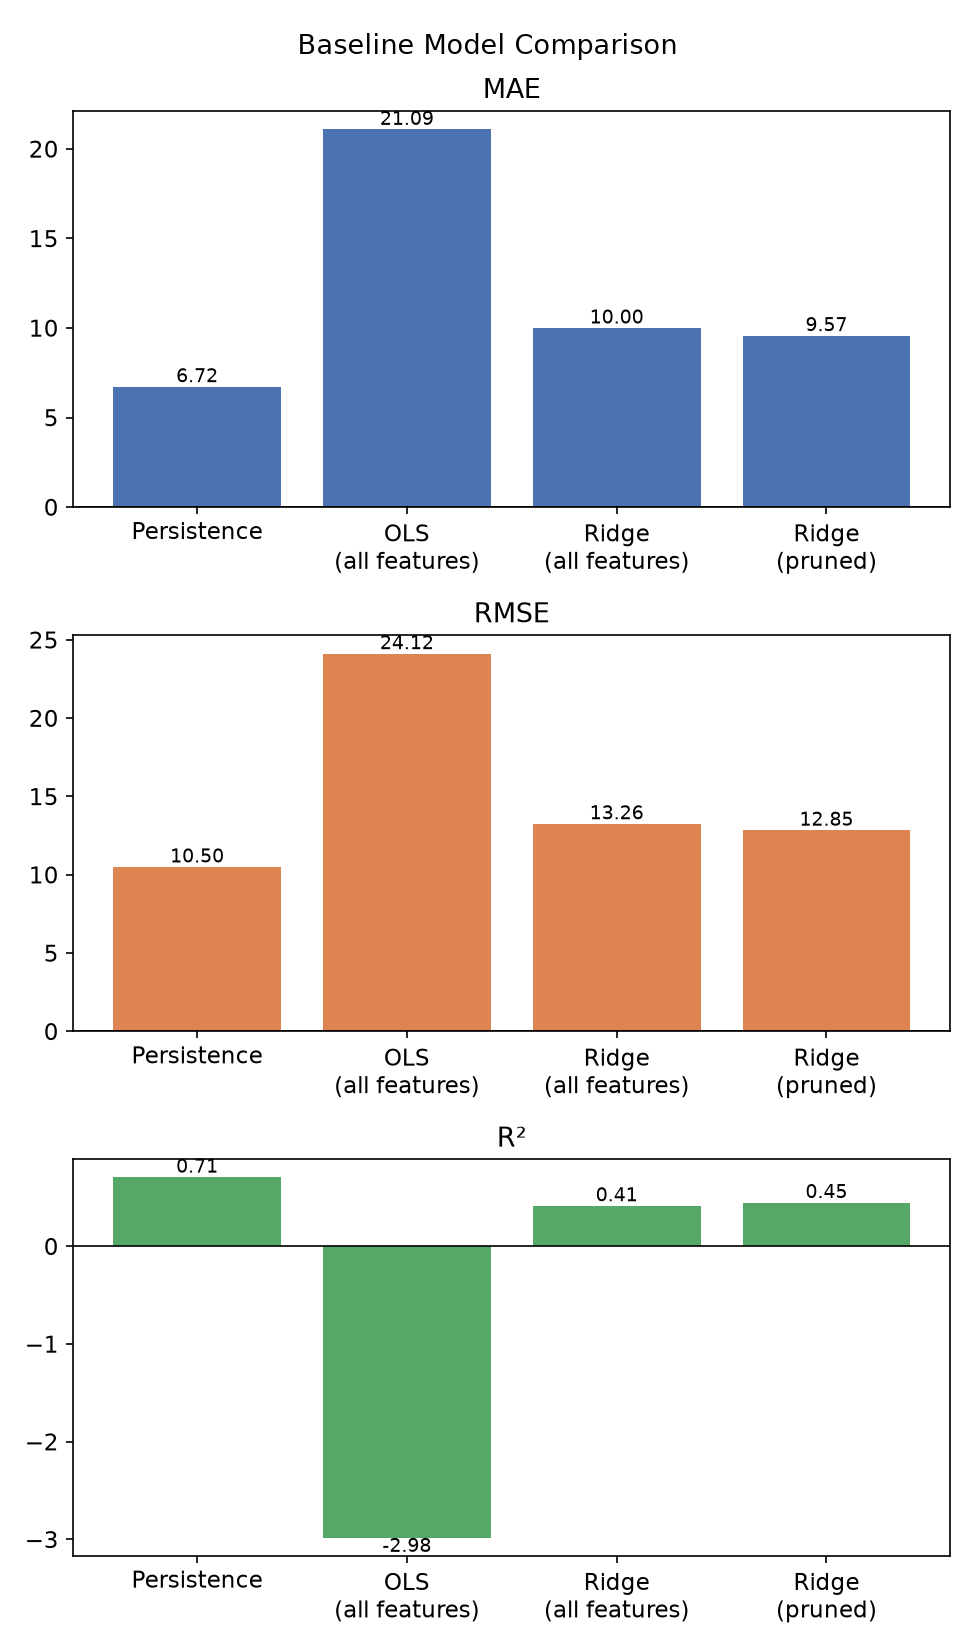
\includegraphics[width=0.92\textwidth]{src/images/figures/fig_model_comparison.png}
    \caption{Baseline model comparison}
    \label{fig:model_comparison}
\end{figure}


The final Ridge model remains slightly below the persistence baseline. This is expected
at this stage: persistence is a strong baseline for one-hour-ahead PM$_{2.5}$ forecasting
since pollution levels change little hour to hour, and a linear model using only a
single station's own history has limited additional signal to extract. The wind-aware
graph structure (Section 5.3) is intended to supply the additional spatial signal --
from neighboring, upwind stations -- needed to meaningfully exceed the persistence
baseline.

\section{Impact of Regularization on Model Generalization}


\begin{table}[H]
    \centering
    \small
    \caption{Impact of Regularization on Model Generalization}
    \label{tab:regularization_generalization_impact}
    \renewcommand{\arraystretch}{1.2}
    \begin{tabularx}{0.94\linewidth}{|X|X|}
        \hline
        \textbf{Configuration} & \textbf{Effect} \\
        \hline
        OLS, all features & Severe overfitting to multicollinear inputs; unstable, unbounded predictions on several stations; mean $R^2 = -2.98$ \\
        \hline
        Ridge ($\alpha=10$), all features & Coefficient instability controlled; mean $R^2 = 0.415$ \\
        \hline
        Ridge ($\alpha=10$), pruned features & Redundant inputs removed in addition to regularization; mean $R^2 = 0.448$, median $R^2 = 0.560$ \\
        \hline
    \end{tabularx}
\end{table}


\begin{figure}[H]
    \centering
    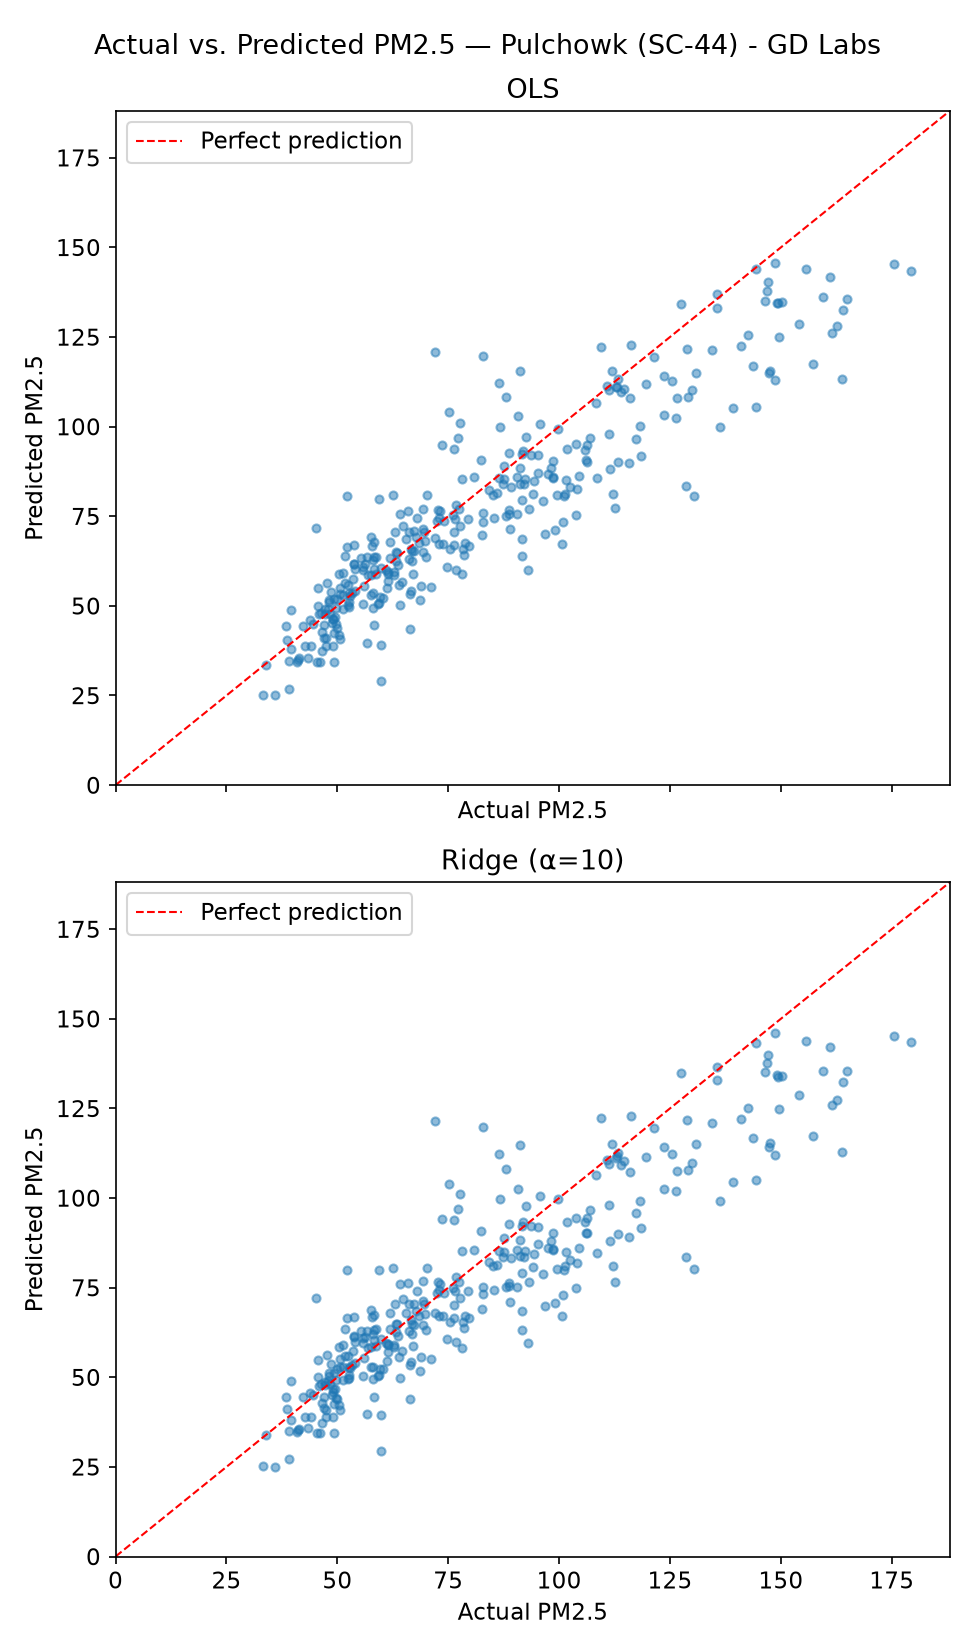
\includegraphics[width=0.92\textwidth]{src/images/figures/fig_ols_vs_ridge_scatter.png}
    \caption{OLS and Ridge prediction comparison}
    \label{fig:ols_vs_ridge}
\end{figure}


\section{Station-wise Performance and Outlier Analysis}


Per-station results for the final Ridge model show a wide but largely healthy spread:

\begin{itemize}
    \item Median $R^2$ across 49 stations: \textbf{0.560} (higher than the mean of 0.448, since the mean is pulled down by a small number of underperforming stations)
    \item 47 of 49 stations achieve a positive $R^2$, most in the 0.3--0.9 range
    \item Best-performing stations ($R^2 > 0.85$): Dabali, Sundarighat, Tarakeswor, Dhathutole
\end{itemize}

\begin{figure}[H]
    \centering
    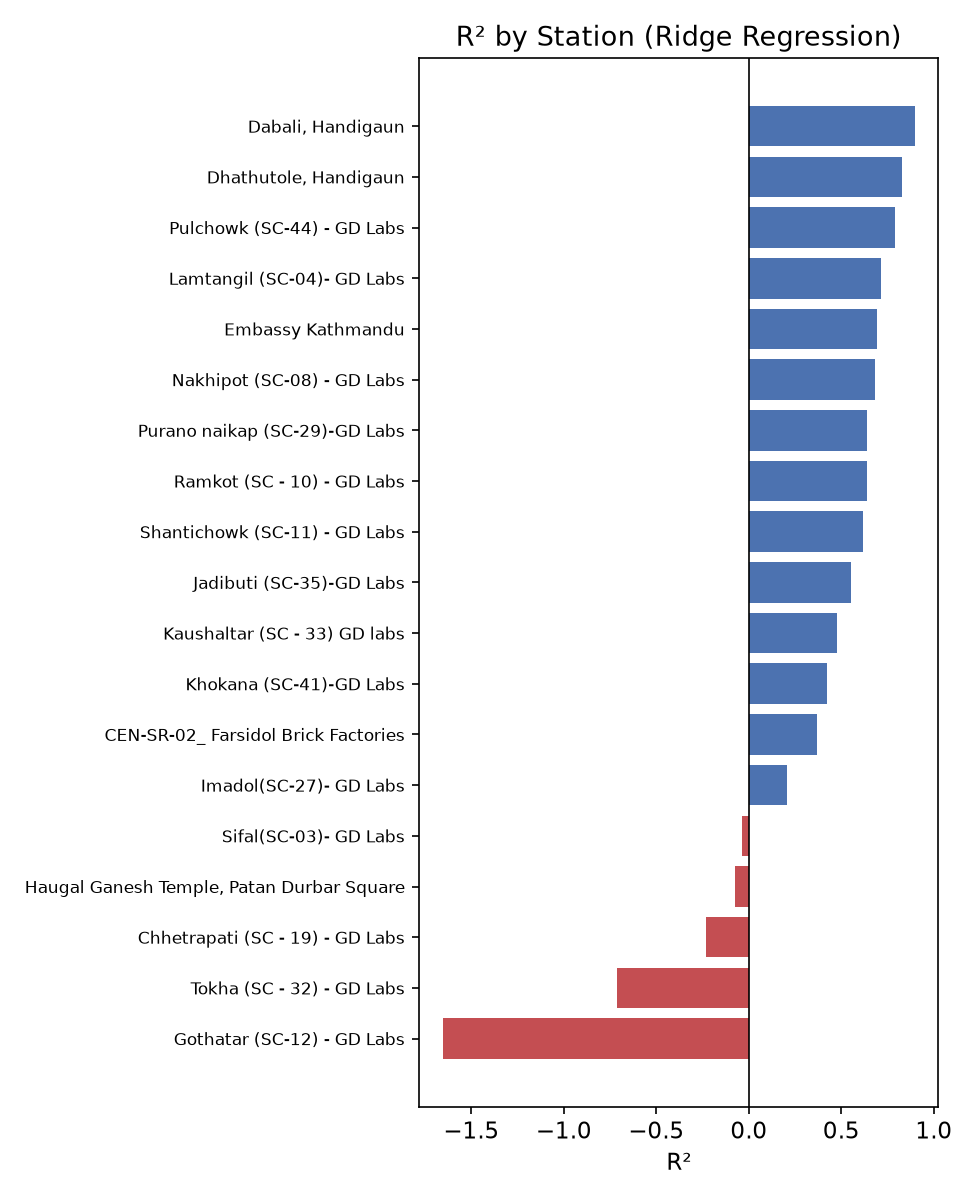
\includegraphics[width=0.92\textwidth]{src/images/figures/fig_station_r2.png}
    \caption{Station-wise $R^2$ performance}
    \label{fig:station_r2}
\end{figure}


One station, \textbf{Gothatar}, remains a clear outlier ($R^2 = -3.32$, MAE = 16.5) despite a
comparatively large training set (1,620 rows) -- traced in Section 6.4 to a large data
gap in its history. Two stations with short monitoring histories -- \textbf{Ramkot} (206
total rows) and \textbf{Sifal} (116 total rows) -- were initially suspected of underperforming
due to insufficient training data; after feature pruning, both achieved reasonable
$R^2$ (0.40 and 0.67 respectively), indicating that multicollinearity, not data volume,
was the dominant issue for most stations.

\section{Timestamp Continuity Findings}


Timestamp continuity validation was run across all 49 prepared station files. Overall
data quality was high: every station exceeded 93\% valid (exactly one-hour) gaps between
consecutive readings, with most stations at 98--99\%.

\begin{figure}[H]
    \centering
    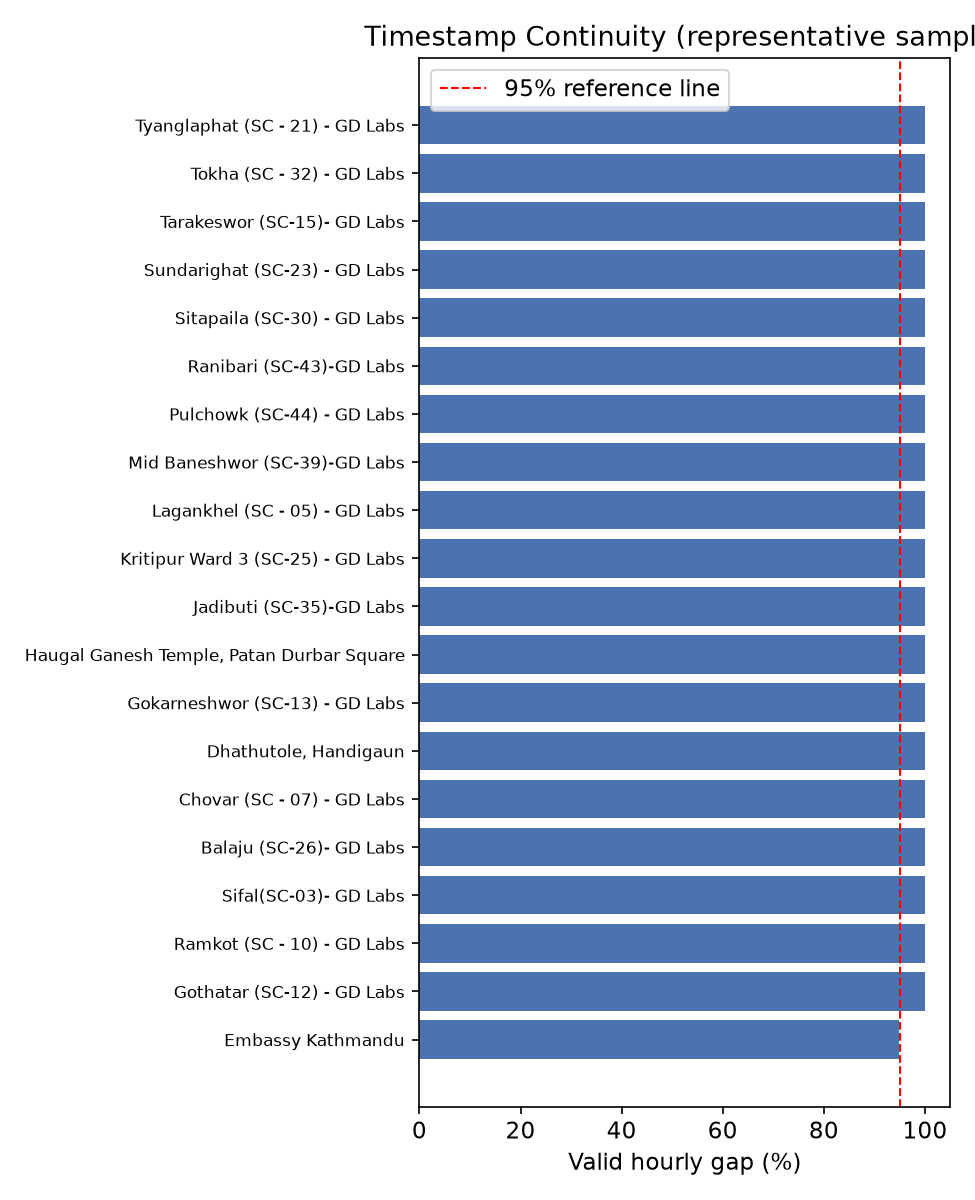
\includegraphics[width=0.92\textwidth]{src/images/figures/fig_timestamp_validity.png}
    \caption{Timestamp validity by station}
    \label{fig:timestamp_validity}
\end{figure}


Notable findings:

\begin{itemize}
    \item \textbf{Gothatar} shows a single gap of approximately 2,906 hours (\textasciitilde{}121 days) despite an otherwise 98.9\% valid-gap rate -- the most likely explanation for its poor model performance, since it plausibly falls near the train/test split boundary and creates a distribution mismatch.
    \item \textbf{Ramkot} has a 1,099-hour (\textasciitilde{}46-day) gap within an already short 206-row history.
    \item \textbf{Sifal} has zero internal gaps (100\% valid hourly spacing) but only 116 total rows -- this station simply began monitoring recently, rather than suffering data-quality issues.
\end{itemize}

\section{Actual vs. Predicted PM$_{2.5}$ Over Time}


\begin{figure}[H]
    \centering
    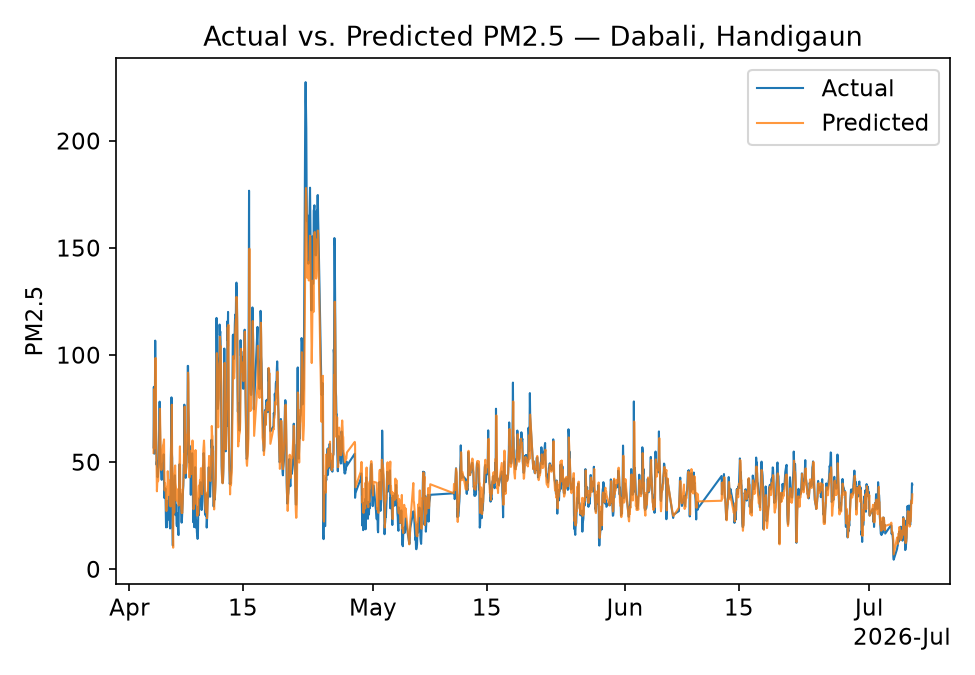
\includegraphics[width=0.92\textwidth]{src/images/figures/fig_timeseries_good_station.png}
    \caption{Actual vs. predicted PM$_{2.5}$ for a representative station}
    \label{fig:timeseries_good_station}
\end{figure}


\begin{figure}[H]
    \centering
    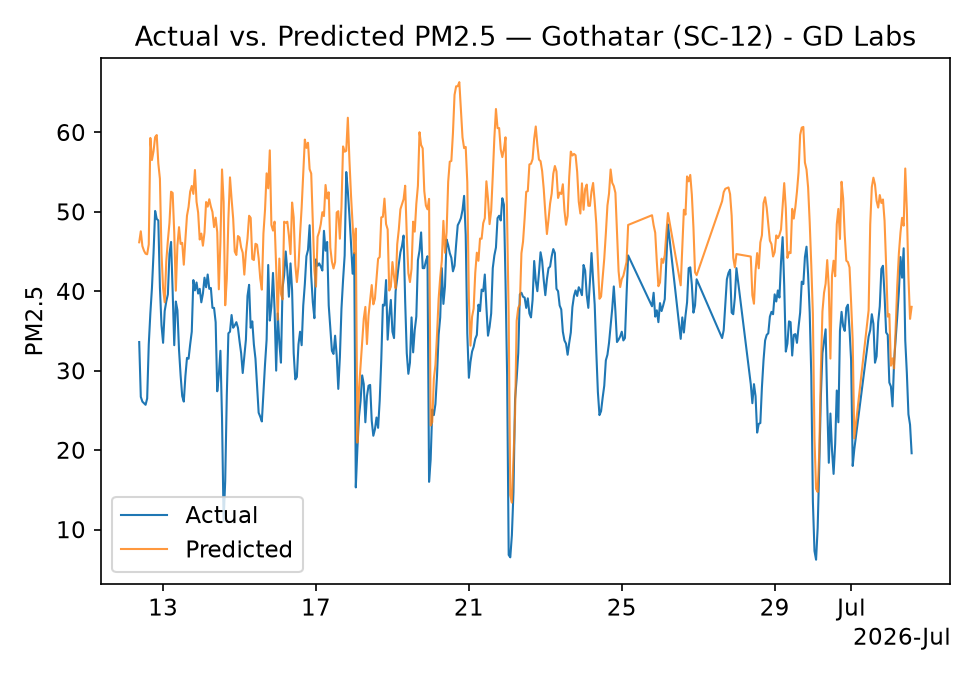
\includegraphics[width=0.92\textwidth]{src/images/figures/fig_timeseries_gothatar.png}
    \caption{Actual vs. predicted PM$_{2.5}$ for Gothatar}
    \label{fig:timeseries_gothatar}
\end{figure}


\section{Summary of Key Findings}


\begin{itemize}
    \item The persistence baseline is a genuinely strong reference point ($R^2$ = 0.708) for one-hour-ahead PM$_{2.5}$ forecasting due to the high hour-to-hour autocorrelation of pollution levels.
    \item An initial OLS linear regression failed catastrophically ($R^2$ = -2.98) due to severe multicollinearity among engineered lag/rolling PM$_{2.5}$ features, not due to a flaw in the underlying modeling approach.
    \item Switching to Ridge regression and pruning redundant features recovered a stable, reasonable baseline ($R^2$ = 0.448 mean / 0.560 median), though it does not yet exceed persistence -- expected at this stage, since a per-station linear model cannot access cross-station wind-driven information.
    \item Data-quality investigation (timestamp continuity validation) explained nearly all station-level outliers, distinguishing genuine data limitations (Gothatar's gap, Ramkot's and Sifal's short histories) from modeling errors.
    \item These findings directly motivate the remaining work: the wind-aware graph and GAT-GRU model are expected to supply the additional cross-station signal needed to exceed the persistence baseline.
\end{itemize}
